\documentclass[final]{thesis}
\usepackage[utf8]{vietnam}
\usepackage{placeins}
\usepackage{amsfonts}
\usepackage{textcomp}
\usepackage{dblfloatfix}
\usepackage{subfig}
\usepackage{lineno}
\usepackage{amssymb}
\usepackage{tabularx,booktabs}
\usepackage{longtable, lipsum}
\usepackage{amsmath}
\usepackage{mathtools}
\usepackage{graphicx}
\usepackage{lscape}
\usepackage{caption}
\usepackage{hyperref}
\usepackage[sorting=ynt]{biblatex}
\usepackage{mathtools}
\usepackage{lipsum}
\usepackage{fancyhdr}
\usepackage{titlesec}
\usepackage{makecell}

% Config reference
\addbibresource{references.bib}

% Setup hype link in thesis
\hypersetup{urlcolor=blue,linkcolor=black,citecolor=black,colorlinks=true} 
\DeclarePairedDelimiter\bra{\langle}{\rvert}
\DeclarePairedDelimiter\ket{\lvert}{\rangle}
\DeclarePairedDelimiterX\braket[2]{\langle}{\rangle}{#1 \delimsize\vert #2}


% Config information thesis
\upperuniname{ĐẠI HỌC QUỐC GIA THÀNH PHỐ HỒ CHÍ MINH}
\uniname{TRƯỜNG ĐẠI HỌC CÔNG NGHỆ THÔNG TIN}
\deptname{KHOA MẠNG MÁY TÍNH VÀ TRUYỀN THÔNG}
\stumajor{KỸ SƯ NGÀNH AN TOÀN THÔNG TIN}
\title{TÌM HIỂU CÁC THUẬT TOÁN ẨN DỮ LIỆU TRONG TẬP TIN VIDEO}
\titleen{TÌM HIỂU CÁC THUẬT TOÁN ẨN DỮ LIỆU TRONG TẬP TIN VIDEO}
\supervisor{GIẢNG VIÊN HƯỚNG DẪN}
\supervisorname{TS. NGUYỄN TẤN CẦM}
\stuname{NGUYỄN HỒNG SƠN \\TÔ TRỌNG NGHĨA }
\stunamewithid{NGUYỄN HỒNG SƠN - 220202022\\TÔ TRỌNG NGHĨA - 220202019}
\reporttime{NĂM 2023}

% Begin thesis
\begin{document}

\coverpage%
% \secondcoverpage%

% % Begin above main thesis
\frontmatter
% \chapter*{\centering\Large{Thông tin hội đồng chấm khóa luận tốt nghiệp}}
\addcontentsline{toc}{chapter}{Thông tin hội đồng chấm khóa luận tốt nghiệp}
Hội đồng chấm khóa luận tốt nghiệp, thành lập theo Quyết định số 463/QĐĐHCNTT ngày 23 tháng 7 năm 2021 của Hiệu trưởng Trường Đại học Công nghệ
Thông tin.
\begin{center}
    \begin{tabular}{ p{.4\textwidth} p{.3\textwidth}} 
        1. TS. Nguyễn Tuấn Nam  & Chủ tịch \\
        2. ThS. Nguyễn Duy   & Ủy viên \\ 
        3. ThS. Trần Hồng Nghi & Thư ký \\ 
    \end{tabular} 
\end{center}



% \chapter*{\centering\Large{Lời cảm ơn}}
\addcontentsline{toc}{chapter}{Lời cảm ơn}
Không ai đạt được điều gì đó to lớn mà không nhờ sự giúp đỡ của những
người xung quanh, cho dù là trực tiếp hay gián tiếp đi nữa. Để hoàn thành được
khóa luận này, nhóm tác giả may mắn nhận được nhiều sự giúp đỡ và hỗ trợ từ
quý thầy, cô, anh chị, bạn bè và người thân. Nhóm tác giả xin dành những trang
đầu tiên này để bày tỏ lòng tri ân của mình tới tất cả mọi người, những người đã
đồng hành cùng nhóm trong khoảng thời gian vừa qua. \\
\indent Đầu tiên, nhóm tác giả xin gửi lời cảm ơn sâu sắc đến toàn thể các thầy cô
của Trường Đại học Công nghệ Thông tin nói chung và các thầy cô khoa Mạng
máy tính và Truyền thông nói riêng. Nhờ những kiến thức quý giá mà thầy cô đã
truyền đạt, cũng như việc hỗ trợ tận tình trong suốt khoảng thời gian thực hiện,
nhóm đã hoàn thành khóa luận và đạt được các kết quả đáng ghi nhận.
Nhóm tác giả xin đặc biệt cảm ơn TS. Nguyễn Ngọc Tự là người đã truyền
cảm hứng, tận tình hướng dẫn và hỗ trợ tận tình về kiến thức, tạo môi trường thuận
lợi để nhóm có thể học hỏi, trao đổi với các bạn, các em trong nhóm nghiên cứu.
Đây là những kiến thức, kinh nghiệm quý giá, không chỉ có tác dụng trong khóa
luận tốt nghiệp này mà còn trong khoảng thời gian làm việc trong chặng đường
tiếp theo. \\
\indent Trong giai đoạn dịch bệnh khó khăn, tình hình ngày càng phức tạp, dù có
khó khăn trong nhiều công việc, nhóm nhận được nhiều sự giúp đỡ và động viên
từ thầy cô và bạn bè. Đây là động lực to lớn thúc đẩy nhóm làm việc trong suốt
quá trình tìm hiểu và hoàn thành khóa luận này. \\
\indent Cuối cùng, nhóm tác giả không quên bày tỏ lòng tri ân đến gia đình và người
thân, những người đã luôn là những hậu phương vững chắc và luôn ủng hộ từng
quyết định mà nhóm đưa ra. \\
\indent Mặc dù đã nỗ lực rất nhiều để luận văn được hoàn thiện nhất, song khó có
thể tránh khỏi thiếu sót và hạn chế. Kính mong nhận được sự thông cảm và ý kiến
đóng góp từ quý thầy cô và các bạn.\\

\begin{flushright}
\textit {TP. Hồ Chí Minh, ngày 12 tháng 7 năm 2021} \\
\textit {Nhóm tác giả}
\end{flushright}


\tableofcontents
\clearpage
\listoffigures

\clearpage

\listoftables





\clearpage

% Begin main thesis, start page numbering
\counterwithin{equation}{chapter}
\counterwithin{table}{chapter}
\counterwithin{figure}{chapter}
% \numberwithin{figure}{section}
\setcounter{secnumdepth}{3}
\mainmatter
\fancyhf{}
\fancyfoot[C]{\thepage}
% \include{chapters/main/summary.tex}

% Config page header
\if @twoside
  \fancyhead[EL,OR]{\bfseries\nouppercase\rightmark}
\else
  \fancyhead[R]{\bfseries\nouppercase\rightmark}
\fi

% Main chapter in thesis
\chapter{Tổng quan} 
\label{sec_introduction}

"Steganography" là thuật ngữ dùng để chỉ kỹ thuật giấu một lượng thông tin số nhất định vào một phương tiện đa phương tiện khác. Sự khác biệt giữa Cryptography và Steganography nằm ở việc thông tin Cryptography thường rõ ràng với người truy cập, trong khi thông tin Steganography (được giấu trong một "vật mang thông tin") thì không thể thấy rõ bởi người truy cập do tính chất ẩn của thông tin được giấu. 

Kĩ thuật ẩn thông tin thường có 2 hướng nghiên cứu chính, đó là Giấu tin mật (Steganography) nhằm bảo vệ thông tin được ẩn trong "vật mang tin" và Thủy vân số (Digital watermarking) nhằm bảo vệ chính "vật mang tin". Thủy vân số thường gồm gồm 2 loại và thủy vân số hữu hình và thủy vân số vô hình. Các phương pháp trong Steganography có thể áp dụng trong thủy vân số vô hình vì mục tiêu chung đều là ẩn thông tin. Vì vậy, trong đồ án này, chúng tôi sẽ trình bày về Video steganography là chính, cụ thể hơn và trong miền dữ liệu thô (raw video).

\section{Định dạng tập tin Video}
Định dạng video là cách mà dữ liệu video được mã hóa và lưu trữ trong một tệp số. Quá trình này bao gồm nén và sắp xếp thông tin hình ảnh và âm thanh để tạo ra một tệp video có thể phát được. Lựa chọn định dạng video ảnh hưởng đến kích thước tệp, chất lượng, khả năng tương thích và khả năng phát lại của video. 
Video Steganography có thể được thực hiện bằng cách sử dụng bất kỳ video nào có sẵn trên internet hoặc tự làm qua điện thoại. Tuy nhiên, theo quan điểm của nhà nghiên cứu, việc triển khai kỹ thuật ghi video thành công đôi khi đòi hỏi kiến thức về một định dạng video cụ thể (tiêu chuẩn mã hóa). Có nhiều tiêu chuẩn mã hóa video khác nhau như H.120, H.261, MPEG-1, MPEG2, MPEG-4, H.264, H.265,...

H.260 là tiêu chuẩn mã hóa video đầu tiên được giới thiệu vào năm 1984. Tiêu chuẩn mã hóa này không được sử dụng trong thực tế do hiệu suất kém. Sau đó, H.261 là tiêu chuẩn mã hóa video thực tế đầu tiên được phát triển dựa trên nén DCT bù chuyển động (motion compensated DCT compression). Tiêu chuẩn tiếp theo là MPEG-1 được phát triển bởi Motion Picture Experts Group (MPEG) để nén VHS (Video Home System). Nó vượt trội so với H.261 về chất lượng khi hoạt động ở tốc độ bit cao. Tiêu chuẩn đã thêm chuyển động nửa pixel và dự đoán chuyển động hai chiều vào H.261. Hơn nữa, MPEG-1 đã bị vượt qua bởi MPEG-2/H.262 được sử dụng cho các định dạng quảng bá ở tốc độ dữ liệu cao và được sử dụng rộng rãi cho tiêu chuẩn DVD. MPEG-2 có thể hỗ trợ hiệu quả các hình ảnh quét xen kẽ với dải tốc độ bit rộng. Tiêu chuẩn tiếp theo là MPEG-4/H.263 được phát triển vào năm 1999 còn được gọi là MPEG-4 Phần 2 đã tạo ra những tiến bộ hơn nữa trong nén video. Tiêu chuẩn này cung cấp các tính năng như mã hóa hình dạng được phân đoạn, kích thước khối thay đổi, mã hóa nội bộ dự đoán không gian, khả năng mở rộng không gian và thời gian, bù chuyển động khối chồng chéo,… Trong số các tiêu chuẩn này MPEG-1, MPEG-2, MPEG-4 đã được các nhà nghiên cứu về kỹ thuật giấu video sử dụng và hiện tại, tiêu chuẩn mã hóa video được sử dụng phổ biến nhất cho kỹ thuật giấu video là H.264/AVC.

Các khung hình video được phân chia thành các khối bằng cách sử dụng kích thước khối thay đổi và dự đoán khối được thực hiện dựa trên các khối lân cận của nó (khung hình trước đây hoặc khung hình trong tương lai). Pixel hữu hình được sử dụng để trừ đi dự đoán để thu được phần còn lại và dữ liệu pixel còn lại này được biến đổi bằng DCT số nguyên. Các hệ số nguyên DCT được lượng tử hóa và sau đó mã hóa entropy được thực hiện để biến đổi nó thành một dòng bit. Đây là tiêu chuẩn mã hóa video được sử dụng rộng rãi nhất trên các nguồn internet phát trực tuyến như Netfix, YouTube và các nguồn web khác. Định dạng mã hóa video hiện đại của ITU-T, VCEG là Mã hóa video hiệu quả cao (HEVC) được giới thiệu vào năm 2013. HEVC, còn được gọi là H.265/HEVC nhằm giải quyết về cơ bản tất cả các ứng dụng phổ biến của H. 264/AVC. Ngoài ra, HEVC tập trung vào việc tăng cường sử dụng các kiến trúc xử lý song song và tăng độ phân giải video. Tiêu chuẩn mã hóa video này được thiết kế đặc biệt để đáp ứng nhu cầu về độ phân giải video độ phân giải cao. H.265/HEVC sử dụng các phép biến đổi DCT và DST số nguyên với kích thước khối có thể thay đổi trong khoảng từ 4×4 đến 32×32.

\section{Video steganography là gì}
Video Steganography là quá trình ẩn thông tin bí mật bên trong video. Thông tin bí mật có thể là bất kỳ phương tiện nào như văn bản, âm thanh, hình ảnh, video và tệp nhị phân và video của nhà cung cấp dịch vụ có thể ở dạng thô/nén ở bất kỳ định dạng nào.

Khả năng không bị phát hiện là một thành phần bắt buộc của kỹ thuật giấu tin. Nền tảng này được minh họa thông qua Bài toán người tù (Prisoners’ Problem).

\begin{figure*}[!h]
    \centering
    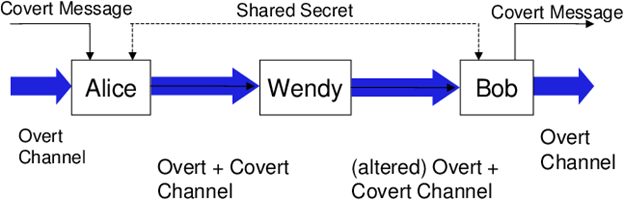
\includegraphics[width=0.9\textwidth]{graphics/chapter-1/Prisoner'problem.png}
    \caption{Tổng quan Bài toán người tù}
    \label{fig:prisonerProblem}
\end{figure*}

Hai cá nhân (Alice và Bob) bị cầm tù. Alice và Bob có thể giao tiếp với nhau, nhưng mọi hoạt động giao tiếp của họ đều bị giám sát liên tục bởi một cai ngục (Wendy). Alice và Bob muốn ấp ủ một kế hoạch trốn thoát, để làm được điều này, họ sẽ sử dụng kỹ thuật ghi mật mã để liên lạc bí mật. Điều quan trọng là thông tin liên lạc của họ không thể bị phát hiện, vì chỉ cần có sự hiện diện của một tin nhắn bí mật sẽ cảnh báo cho Wendy.

\section{Phân loại}
Mức phân loại đầu tiên dựa trên định dạng của video che (cover video). Video che được xem xét thuộc miền thô (Raw domain) hay miền nén (compressed domain). Các video miền thô được phân loại thành miền không gian (spatial domain) và miền biến đổi (transform domain). Phương pháp thay thế Bit ít quan trọng nhất (Least Significant Bits - LSB) và các phương pháp quan trọng khác được bao gồm trong miền không gian. Biến đổi Wavelet rời rạc (DWT) và Biến đổi Cosine rời rạc (DCT) là các phương pháp biến đổi được sử dụng rộng rãi để biến đổi các video che thành miền biến đổi. Sau khi biến đổi video thành miền biến đổi, việc nhúng thông tin bí mật được thực hiện. Trong miền nén, ghi video sử dụng video che nén. Video được nén có ít dung lượng lưu trữ hơn so với video thô và quá trình nhúng diễn ra trong hoặc sau quá trình nén video. Vectơ chuyển động, chế độ dự đoán nội bộ, mô-đun mã hóa entropy, và các kỹ thuật DCT/DST là các phương pháp ghi video được sử dụng rộng rãi trong miền nén. 

Video Steganography có ứng dụng của nó trong các lĩnh vực/lĩnh vực khác nhau, nơi thường sử dụng giao tiếp bí mật. Các lĩnh vực phổ biến mà kỹ thuật giấu tin video được sử dụng là các cơ quan tình báo, quân đội, ngành y tế và đa phương tiện. Các cơ quan tình báo luôn thích giao tiếp bí mật khi họ giao tiếp bên trong cũng như bên ngoài cơ quan. Video Steganography được sử dụng rộng rãi trong trường hợp này khi chúng có thể che giấu sự tồn tại của thông điệp bí mật khỏi kẻ tấn công. Tương tự như các cơ quan tình báo, các tổ chức quân sự cũng đang sử dụng rộng rãi các kỹ thuật steganography để che đậy thông tin liên lạc của họ. Bởi vì việc tiết lộ trái phép dữ liệu bí mật có thể dẫn đến các vấn đề về an ninh quốc gia. Lĩnh vực y tế cũng đã được hưởng lợi từ việc áp dụng kỹ thuật ghi video. Sự tiến bộ hiện nay trong lĩnh vực y tế đã làm cho việc lưu trữ thông tin của bệnh nhân ở dạng kỹ thuật số. Hơn nữa, thông tin này được lưu trữ trên đám mây và có thể được chuyển đến bệnh nhân tương ứng hoặc nhà cung cấp dịch vụ chăm sóc sức khỏe được ủy quyền với sự trợ giúp của kết nối internet. Truyền dữ liệu y tế qua internet là một vấn đề nghiêm trọng vì bất kỳ sự mất mát dữ liệu nào xảy ra do các cuộc tấn công mạng đều có thể ảnh hưởng tiêu cực đến sức khỏe của bệnh nhân. Ngành y tế đang sử dụng các kỹ thuật ghi video để che giấu thông tin cá nhân của họ khỏi các thực thể trái phép khi nó được chuyển qua các kênh liên lạc. Ngoài ra, kỹ thuật ghi video được sử dụng để bảo vệ quyền riêng tư của các cá nhân được ủy quyền được phát hiện trong các chuỗi video do camera giám sát ghi lại. Dữ liệu của các cá nhân được nhúng bên trong các chuỗi video từ camera giám sát. Các đặc điểm chính của bất kỳ phương pháp steganography nào là không thể nhận thấy, bảo mật, mạnh mẽ và khả năng che giấu. Luôn có sự thỏa hiệp giữa tính bảo mật, tính mạnh mẽ và khả năng che giấu của các phương pháp lưu trữ dữ liệu.

\begin{figure*}[!h]
    \centering
    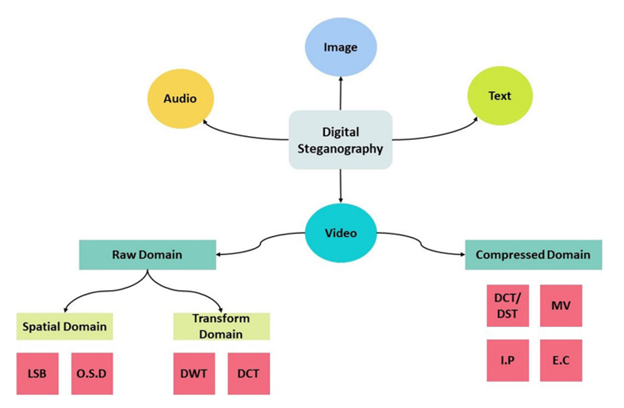
\includegraphics[width=0.9\textwidth]{graphics/chapter-1/Classif_VideoSte.png}
    \caption{Phân loại các dạng Video Steganography}
    \label{fig:classifi}
\end{figure*}

\subsection{Video steganography trong miền thô (Raw domain)}
Các phương pháp ghi video dựa trên miền thô coi video che (cover video) là một chuỗi các khung và thao tác nhúng dữ liệu được áp dụng cho từng khung riêng biệt. Quy trình nhúng dữ liệu chung trong miền thô được hiển thị trong hình \ref{fig:Process_rawdomain} bên dưới. 

\begin{figure*}[!h]
    \centering
    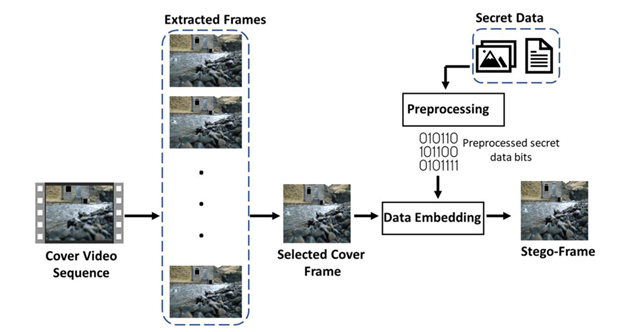
\includegraphics[width=0.9\textwidth]{graphics/chapter-1/Process_rawdomain.png}
    \caption{Quy trình nhúng dữ liệu chung trong miền thô}
    \label{fig:Process_rawdomain}
\end{figure*}

Ban đầu, chuỗi video che (cover video sequence) được chuyển đổi thành nhiều khung hình. Sau đó, dữ liệu bí mật được ẩn bên trong các khung bằng nhiều phương pháp khác nhau. Trong miền thô, dữ liệu bí mật được nhúng trực tiếp vào miền không gian của khung che (cover frame) hoặc khung che được chuyển thành miền tần số (frequency domain) và dữ liệu bí mật được nhúng vào miền tần số. Trước khi nhúng, dữ liệu bí mật phải được tiền xử lý. Nhiều phương pháp đã áp dụng các kỹ thuật mã hóa (encryption techniques), mã sửa lỗi (error-correcting codes),… để xử lý trước dữ liệu bí mật. Quá trình tiền xử lý dữ liệu bí mật được triển khai để đảm bảo tính bảo mật của dữ liệu bí mật ngay cả khi video che bị bất kỳ cuộc tấn công nào hoặc giảm khung hình (frame drops) trong quá trình truyền. 

Phương pháp dựa trên miền thô (raw domain-based method) có thể được phân thành hai loại: ẩn dữ liệu trong miền không gian (Data hiding in spatial domain) và ẩn dữ liệu trong các phương thức miền biến đổi (Data hiding in transform domain).

\begin{itemize}
    \item Ẩn dữ liệu trong miền không gian (Data hiding in spatial domain):
    Các kỹ thuật giấu dữ liệu trong miền không gian sử dụng các giá trị pixel của khung che để giấu dữ liệu bí mật. Nó có nghĩa là các bit dữ liệu bí mật được nhúng trực tiếp vào các giá trị cường độ pixel (pixel intensity values). Các bit ít quan trọng nhất (The least significant bits - LSB) hay  thay thế LSB (LSB substitution) là một phương pháp phổ biến, trong đó các bit dữ liệu bí mật được nhúng vào các bit ít quan trọng nhất của cường độ pixel che phủ (cover pixels intensities), được sử dụng để ẩn dữ liệu trong miền không gian. 
    \begin{itemize}
        \item Các phương pháp LSB:     
Các phương pháp dựa trên các Bit ít quan trọng nhất là thuật toán thường được sử dụng cho kỹ thuật ghi ảnh, âm thanh và video. Các phương pháp LSB rất đơn giản và hiệu quả. Thông thường, các phương thức LSB được mô tả là các phương thức thay thế k-LSB trong đó k là số bit bí mật có thể được ẩn. Dựa trên thuật toán nhúng, giá trị của k được thay đổi. Khả năng ẩn của thuật toán nhúng phụ thuộc vào số bit (k) có thể được thao tác trong video che. Tăng số lượng bit để giấu tin có thể tăng khả năng giấu tin nhưng cũng sẽ làm quá tải cho phương tiện mang tin, dẫn đến việc tiết lộ thông tin bí mật. Bảng \ref{tab:LSB_survey} thể hiện một số nghiên cứu sử dụng phương pháp LSB. Trong bảng \ref{tab:LSB_survey}, \textbf{Imp} thể hiện cho tính không thể nhận thấy; \textbf{Rob} thể hiện cho độ mạnh mẽ; và \textbf{Cap} thể hiện cho khả năng che giấu của thuật toán.

\begin{table}[!h]
\caption{Các nghiên cứu sử dụng phương pháp LSB} 
\label{tab:LSB_survey}
\centering
\resizebox{\textwidth}{!}{%
\begin{tabular}{|c|c|c|c|c|c|}
\hline
\textbf{Year} & \textbf{Method}                               & \textbf{Imp} & \textbf{Rob} & \textbf{Cab} & \textbf{Remarks}         \\ \hline
2019 & 2-LSB \cite{1_younus2019video}                            & + & - & N/A         & Security   is not tested       \\ \hline
2011 & 1-LSB \cite{2_ramalingam2011stego}                            & + & - & N/A         & Security   is not tested       \\ \hline
2011 & 4-LSB  \cite{3_hu2011novel}                           & + & - & 1.5   bpp   & No   obvious visual distortion \\ \hline
2012 & Hash-LSB \cite{4_dasgupta2012hash}                        & + & - & 2.6   bpp   & Low                            \\ \hline
2014 & Hash-LSB \cite{5_kaur2014improved}                         & + & - & 100\%       & Security   is not tested       \\ \hline
2017 & Spiral LSB \cite{6_jha2017video}                      & + & - & 25\%        & Low   hiding capacity          \\ \hline
2020 & Adaptive 4-LSB \cite{7_mstafa2020new}               & + & + & 0.069   bpp & Low   embedding capacity       \\ \hline
2013 & 3–3-2   LSB and Genetic algorithm \cite{8_dasgupta2013optimized} & + & - & 8   bpp     & Security   is low              \\ \hline
2010          & LSB   replacement  and directed graph patterns \cite{9_bhattacharyya2010directed} & -                         & -                   & 2560   KB         & Security   is not tested \\ \hline
\end{tabular}%
}
\end{table}

Một pixel duy nhất trong khung của video bao phủ có từ 8 đến 24 bit dựa trên định dạng của video. Các khung màu xám có 8 bit trong khi một khung màu sắc có 24 bit. Một khung màu sắc bao gồm 3 kênh (RGB) và mỗi kênh bao gồm 8 bit cho mỗi pixel. Tương tự, một khung bí mật RGB của video bao gồm 8 bit cho mỗi pixel cho tất cả 3 kênh. Các bit ít quan trọng nhất của khung bao phủ được thay thế bằng các bit quan trọng nhất của khung bí mật. Trong quá trình trích xuất, các bit LSB của ảnh Stego được lấy ra và các bit 0 được thêm vào để thu được một xấp xỉ thông tin bí mật như ý.
        \item Các phương pháp miền không gian khác:

Hầu hết các kỹ thuật ghi video cho video thô trong miền không gian đều dựa vào sự thay thế LSB để nhúng dữ liệu bí mật. Bên cạnh đó, một số công trình được đề xuất trong thập kỷ qua đã sử dụng các phương pháp không phải LSB để ẩn dữ liệu bí mật trong miền không gian của video thô.


Hầu hết LSB và các phương pháp miền không gian khác đều đạt được khả năng che giấu dữ liệu cũng như khả năng che giấu dữ liệu chấp nhận được. Tuy nhiên, tính mạnh mẽ của các phương pháp được đề xuất là một mối quan tâm và nhiều phương pháp chưa tiến hành bất kỳ phân tích định lượng nào để đánh giá tính mạnh mẽ của chúng. Hầu hết các phương pháp dựa trên miền không gian dễ bị tấn công phân tích dữ liệu và không đủ mạnh để chống lại các cuộc tấn công nén (compression attack) cũng như tấn công nhiễu (noise attack).

    \end{itemize}
    \item Ẩn dữ liệu trong miền biến đổi (Data hiding in transform domain):
    Không giống như phương pháp dựa trên miền không gian nhúng trực tiếp dữ liệu bí mật vào cường độ pixel thô của pixel che (cover pixel), phương pháp dựa trên miền biến đổi biến đổi các khối của khung che trong miền không gian sang miền biến đổi. Sau đó, dữ liệu bí mật được nhúng vào các bit có ý nghĩa nhỏ nhất của hệ số biến đổi. Quy trình chung của việc ẩn dữ liệu trong miền biến đổi được thể hiện trong Hình \ref{fig:Process_transform}. Biến đổi wavelet rời rạc (Discrete Wavelet Transform - DWT) và biến đổi cosine rời rạc ( Discrete Cosine Transform - DCT) là hai hàm biến đổi được sử dụng chủ yếu trong kỹ thuật ghi video.

\begin{figure*}[!h]
    \centering
    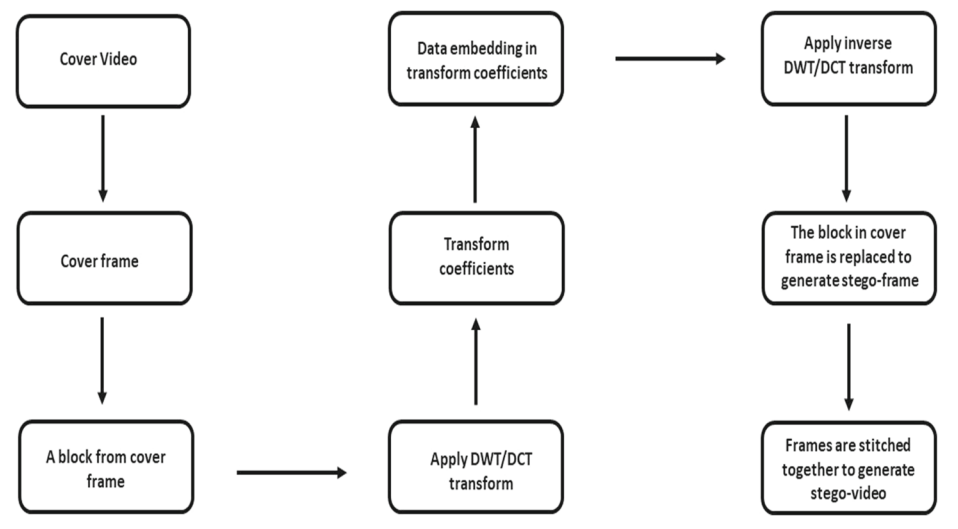
\includegraphics[width=0.9\textwidth]{graphics/chapter-1/transform_overview.PNG}
    \caption{Quy trình nhúng dữ liệu chung trong miền biến đổi}
    \label{fig:Process_transform}
\end{figure*}

    \begin{itemize}
        \item Biến đổi wavelet rời rạc (Discrete Wavelet Transform - DWT):
Một kỹ thuật miền biến đổi khác được sử dụng cho kỹ thuật ghi video là DWT, trong đó quá trình nhúng được thực hiện bằng cách phân tách các khung thành các cấp độ khác nhau. Mỗi cấp độ được chia thành bốn phần tần số, tức là LL, LH, HL và HH trong đó chỉ có một (LL) là thành phần tần số cấp thấp và ba thành phần còn lại là thành phần tần số cấp cao. Nói chung, băng con/thành phần LL được phân tách lặp lại thành các cấp độ cao hơn (Faragallah 2013); tuy nhiên, các băng con khác cũng có thể được phân tách thành các mức khác nhau. Kết quả triển khai phân tách 2D DWT một cấp và hai cấp (băng con LL) trên khung của định dạng video CIF (Định dạng trung gian chung) từ tập dữ liệu dấu vết phổ biến (Reisslein 2012) với độ phân giải 352×288 được hiển thị trong Hình .12.
DWT là một kỹ thuật toán học thường được sử dụng trong xử lý tín hiệu và nén ảnh. Trong phép biến đổi DWT hai chiều, một ảnh gốc I sẽ được phân tích thành bốn băng tần có kích thước bằng $1/2$ ảnh gốc: LL (low frequency component in horizontal and vertical direction), LH (low frequency component in horizontal direction and high frequency in vertical direction), HL (high frequency component in horizontal direction and low frequency in vertical direction), HH (high frequency component in horizontal direction and high frequency in vertical direction).

        \item Biến đổi cosine rời rạc ( Discrete Cosine Transform - DCT):

DCT cũng là một chức năng biến đổi giống như DWT, chia hình ảnh thành các băng con quang phổ. Sự khác biệt chính giữa DCT và DWT là loại trước đó tạo ra nhiều dải tần hơn và cung cấp độ phân giải tần số cao hơn. Tuy nhiên, DWT tạo ra một vài dải tần số và cung cấp độ phân giải không gian cao. Một số lượng đáng kể các tác phẩm trong tài liệu đã sử dụng miền DWT để nhúng dữ liệu bí mật vào các video thô. Không giống như DWT, miền DCT không được sử dụng thường xuyên trong tài liệu để ẩn dữ liệu bí mật bên trong video thô . Mặt khác, các phương pháp ghi video được đề xuất trong miền nén đã sử dụng rộng rãi miền DCT để ẩn dữ liệu bí mật.

    \end{itemize}
\end{itemize}

Bảng \ref{tab:DCT_DWT_survey} thể hiện một số nghiên cứu sử dụng phương pháp DCT và DWT. Trong bảng \ref{tab:DCT_DWT_survey}, \textbf{Imp} thể hiện cho tính không thể nhận thấy; \textbf{Rob} thể hiện cho độ mạnh mẽ; và \textbf{Cap} thể hiện cho khả năng che giấu của thuật toán.

\begin{table}[!h]
\centering
\caption{Các nghiên cứu sử dụng phương pháp DCT và DWT} 
\label{tab:DCT_DWT_survey}
\resizebox{\textwidth}{!}{%
\begin{tabular}{|c|c|c|c|c|c|}
\hline
\textbf{Year} &
  \textbf{Method} &
  \textbf{Imp} &
  \textbf{Rob} &
  \textbf{Cab} &
  \textbf{Remarks} \\ \hline
2014 & DWT,   DCT \& LSB \cite{11_ahmed2014information} & + & + & 1.8   KB    & Security   is not tested                       \\ \hline
2016 & DWT   \& LSB \cite{12_kolakalur2016wavelet}      & + & - & N/A         & Evaluated   in multiple video formats          \\ \hline
2017 &
  DWT   \& LSB \cite{13_sushmitha2017approach} &
  + &
  - &
  N/A &
  Able   to hide multiple videos inside single video with minimal visual distortion \\ \hline
2010 & DWT \cite{14_lu2010effective}              & + & + & N/A         & Biometric   image sets are hidden inside video \\ \hline
1997 & DCT \cite{15_swanson1997data}               & + & + & 74.97   KB  & Security   is not tested                       \\ \hline
2019 & 1D-DCT \cite{16_rabie2019pixogram}            & + & + & 16.64   bpp & Security   is not tested                       \\ \hline
2017 &
  Adaptive   method (DWT \& DCT) \cite{17_mstafa2017robust} &
  + &
  + &
  3.40\% &
  Secure   against state of art steganalysis attacks. \\ \hline
\end{tabular}%
}
\end{table}

\subsection{Video steganography trong miền nén (Compressed domain)}
Phần lớn các phương pháp ghi video để ẩn dữ liệu trong miền thô đều đơn giản và dễ thực hiện. Tuy nhiên, chúng dễ bị tấn công hơn, đặc biệt là các cuộc tấn công nén. Hơn nữa, hiện tại, các video ở dạng nén được ưa chuộng hơn để lưu trữ cũng như truyền qua internet. Video nén cần ít dung lượng lưu trữ hơn so với video không nén. Và việc truyền video ở dạng nén qua internet sẽ nhanh hơn và cần ít băng thông hơn. Trong bối cảnh này, các kỹ thuật ẩn dữ liệu trong miền video nén đã trở nên phổ biến trong hai thập kỷ qua. Mặt khác, quá trình nén sẽ loại bỏ dữ liệu video dư thừa và giảm không gian để ẩn nhiều dữ liệu hơn.

Trong miền nén, việc ẩn dữ liệu được thực hiện theo hai cách; ẩn dữ liệu cùng với quy trình mã hóa video và ẩn dữ liệu trong luồng bit được mã hóa. Các kỹ thuật che giấu dữ liệu cùng với quy trình mã hóa video sử dụng các yếu tố cú pháp khác nhau liên quan đến tác vụ mã hóa video để nhúng dữ liệu bí mật. Đối với cách còn lại - các phương pháp ẩn dữ liệu trong luồng bit - sẽ được mã hóa khai thác các mô-đun mã hóa entropy để mang dữ liệu bí mật.

\section{Đặc trưng của Video steganography}
Đánh giá các phương pháp steganography video là rất quan trọng để xác định hiệu suất và hiệu quả của phương pháp. Các tính năng chính được mong đợi từ các phương pháp lưu trữ dữ liệu tốt thường là tính không thể nhận thấy (Imperceptibility), Khả năng che giấu (Hiding capacity), bảo mật (security), Độ mạnh mẽ (Robustness) và khả năng chống lại các cuộc tấn công phân tích dữ liệu khác.
\subsection{Tính không thể nhận thấy (Imperceptibility)}
Khả năng che giấu đo lường khả năng của phương pháp steganography video để nhúng một lượng dữ liệu ẩn vào video mà không gây ra thay đổi đáng kể đối với các đặc điểm chính của video. Phương pháp với khả năng che giấu tốt sẽ cho phép nhúng một lượng lớn dữ liệu mà vẫn duy trì tính tự nhiên và không gây nghi ngờ cho người xem. Tuy nhiên, việc tăng khả năng che giấu có thể dẫn đến việc giảm tính không thể nhận thấy và độ mạnh mẽ của phương pháp.
\subsection{Khả năng che giấu (Hiding capacity)}
Tính không thể nhận thấy là khả năng của phương pháp steganography video để duy trì hình ảnh và âm thanh của video một cách tự nhiên, mà không có sự thay đổi đáng kể. Người xem không nên có khả năng nhận ra sự hiện diện của dữ liệu ẩn trong video một cách dễ dàng. Tính không thể nhận thấy quan trọng để đảm bảo rằng việc ẩn dữ liệu không làm giảm chất lượng trải nghiệm của người xem.
\subsection{Độ mạnh mẽ (Robustness)}
Độ mạnh mẽ của phương pháp steganography video đo lường khả năng của nó chống lại các biến đổi, nhiễu và tấn công mục tiêu mà có thể làm lộ dữ liệu ẩn. Phương pháp mạnh mẽ sẽ duy trì khả năng che giấu và tính không thể nhận thấy ngay cả khi video trải qua các biến đổi như nén ảnh, nén âm thanh, hoặc các cuộc tấn công như tấn công phân tích dữ liệu. Điều này đảm bảo rằng dữ liệu ẩn vẫn an toàn và không bị phát hiện trong các tình huống thực tế.

\chapter{Phân tích ẩn video (Video stegananalysis)}
Trong khi steganography là quá trình che giấu thông tin bí mật, steganalysis là quá trình phá vỡ thuật toán steganography để phát hiện và khám phá thông tin bí mật được nhúng. Steganalysis được phân loại thành Steganalysis tích cực và Steganalysis thụ động. Phân tích ẩn thụ động chỉ phát hiện sự hiện diện của thông tin bí mật, nhưng phân tích ẩn tích cực phát hiện và giải mã/sửa đổi thông tin bí mật ẩn.

Steganalysis rất quan trọng vì hai lý do: 
\begin{itemize}
    \item Cho kỹ thuật ghi ảnh ẩn có thể đảo ngược trong đó phân tích dữ liệu được yêu cầu ở đầu nhận để trích xuất thông tin bí mật được nhúng.
    \item Để ngăn chặn việc chuyển giao thông tin bất hợp pháp.
\end{itemize}
 
 Có rất nhiều công cụ steganography dễ dàng có sẵn trực tuyến, điều này làm cho nhu cầu phân tích trở nên cấp thiết. Ngay cả một người bình thường cũng có thể dễ dàng truy cập các công cụ ghi mật mã và sử dụng chúng để gửi thông tin bí mật và bị cấm mà không gây bất kỳ nghi ngờ nào cho các quan chức chính phủ.

 Nhu cầu phân tích steganalysis là rất lớn, tuy nhiên, phân tích steganalysis không hề dễ dàng. Với việc lựa chọn phương tiện che phủ phù hợp, ngay cả công cụ phân tích ẩn tốt nhất cũng không thể phá vỡ kỹ thuật ghi ẩn. Vì không có bất kỳ thông tin chi tiết nào về phương tiện truyền thông bìa và nếu không có kiến thức đó, việc phá vỡ bản ghi mật là rất khó. Đặc biệt với video là phương tiện truyền thông bìa, việc phân tích dữ liệu có thể là một thách thức vì khó có thể tương quan giữa các video và các đặc trưng. Các phương pháp phân tích mật được phát triển theo ký hiệu rằng các đặc điểm và đặc trưng của phương tiện che phủ được sửa đổi khi thông tin bí mật ăn sâu vào. Nhiều phương pháp phân tích dữ liệu hoạt động bằng cách so sánh các đặc trưng và đặc điểm khác giữa đối tượng stego và đối tượng che phủ.

 Một phân tích kỹ lưỡng về phương pháp ghi ảnh ẩn hiện có và sự tiến bộ của nó là cần thiết để xây dựng công cụ phân tích ảnh. Một phương pháp phân tích ẩn tốt sẽ có thể phá vỡ các cuộc tấn công ẩn khác nhau và một số phương pháp phân tích ẩn hiện có. Steganalysis được chia thành hai loại, cụ thể là Steganalysis cụ thể và Steganalysis phổ quát. Các phương pháp phân tích ẩn cụ thể được phát triển để xử lý một loại phương pháp ẩn giấu cụ thể. Ví dụ, steganography đảo ngược là một phương pháp stegananalysis cụ thể, vì phương pháp này chỉ có thể phá vỡ một phương pháp steganography cụ thể và có thể không hoạt động hiệu quả với các phương pháp steganography khác. Mặt khác, các phương pháp phân tích ẩn phổ biến nhằm mục đích phá vỡ tất cả các phương pháp lưu trữ. Các phương pháp phân tích ẩn cụ thể có thể thực hiện được, trong khi đó, các phương pháp phân tích ẩn phổ quát lại khó thực hiện. Sự phát triển của các phương pháp phân tích ẩn phổ quát nên theo hướng của các công việc trong tương lai. Nỗ lực phát triển một phần mềm duy nhất có khả năng phá vỡ bất kỳ loại steganography nên được đầu tư.

 \section{Kĩ thuật phân tích ẩn}
 Các phương pháp phân tích ẩn được phân loại thành ba loại chính:
 \begin{itemize}
     \item Phân tích ẩn dựa trên chữ ký
     \item Phân tích ẩn thống kê
     \item Phân tích ẩn dựa trên đặc trưng
 \end{itemize}
 
 Phân tích ẩn chữ ký, như tên cho thấy, sử dụng chữ ký (signature) do phương pháp nhúng để lại để phát hiện sự hiện diện của thông tin bí mật. Phân tích ẩn thống kê sử dụng các phương pháp thống kê và công thức toán học để phát hiện và khám phá thông tin bí mật. Các phương pháp phân tích ẩn dựa trên đặc trưng trích xuất các đặc trưng từ video bìa và video ẩn để điều tra sự hiện diện, từ đó, phát hiện ra thông tin bí mật.

 \subsection{Phân tích ẩn dựa trên chữ ký}
 Các phương pháp phân tích chữ ký được chia thành tấn công trực quan và tấn công cấu trúc. Tính năng đầu tiên và quan trọng nhất được mong đợi từ kỹ thuật ghi video là không thể nhận thấy. Sự biến dạng do phương pháp ghi video gây ra phải ở mức tối thiểu, nếu không, dấu vết của thông báo ẩn có thể hiển thị đối với Hệ thống thị giác của con người (Human Visual System - HVS). Các cuộc tấn công thị giác (Visual
attacks) là kỹ thuật phân tích dữ liệu đơn giản có thể phá vỡ kỹ thuật ẩn ảnh bằng cách sử dụng HVS. Khung ẩn và khung bìa được so sánh cạnh nhau bằng mắt thường để kiểm tra bất kỳ thay đổi có thể nhìn thấy nào. Mặc dù các cuộc tấn công bằng hình ảnh rất dễ thực hiện nhưng chúng không đáng tin cậy. Không chỉ độ tin cậy mà cả tính tự động hóa và yêu cầu chuyên gia thực hiện kiểm tra là những nhược điểm khác của việc sử dụng tấn công trực quan.

Các đặc điểm và đặc trưng của video bìa thay đổi sau khi nhúng thông tin bí mật. Một số đặc điểm, đặc trưng và các thành phần cấu trúc khác của video ẩn được tính đến để phát hiện sự hiện diện của thông tin bí mật. Kiểu tấn công phân tích này được gọi là tấn công cấu trúc. Một ví dụ cụ thể có thể kể đến là việc so sánh kích thước tệp. Sau khi nhúng, kích thước tệp của video bìa dễ bị thay đổi. Tương tự như các cuộc tấn công trực quan, các cuộc tấn công cấu trúc không đáng tin cậy và cần có các chuyên gia trong lĩnh vực này. Không phải tất cả các video bị giả mạo đều sẽ thay đổi cấu trúc và có thể thoát khỏi các phương thức tấn công cấu trúc.

\subsection{Phân tích ẩn thống kê}
Phân tích ẩn thống kê sử dụng các giá trị của pixel hình ảnh và phân tích chúng để phát hiện nội dung bí mật. Phân tích ẩn thống kê ưu việt hơn so với phân tích ẩn dựa trên chữ ký. Các phương pháp thống kê sử dụng kiến thức về các giá trị pixel của ảnh và các mô hình toán học để phát hiện và khôi phục thông tin bí mật. Phân tích ẩn thống kê có thể được nhóm thành phân tích Biểu đồ, Tấn công Chi-Square, Phân tích ẩn RS, nhúng LSB, phân tích cặp pixel khớp LSB, phân tích mặt phẳng Bit, nén JPEG và phân tích ẩn miền biến đổi.

Phân tích ẩn biểu đồ phân tích biểu đồ của khung video bìa và khung video stego để phát hiện sự hiện diện của thông tin bí mật. Biểu đồ là biểu diễn đồ họa của các giá trị pixel của hình ảnh dựa trên phân phối. Khi một video bìa được điều khiển để nhúng thông tin bí mật, biểu đồ của video stego bị ảnh hưởng, Việc nhúng thông tin bí mật có thể không nhìn thấy được bằng mắt thường, nhưng khi biểu đồ này được vẽ và so sánh với video bìa gốc, ngay cả thao tác nhỏ nhất cũng có thể được phát hiện.

Kiểm tra Chi-square là một kỹ thuật phân tích dữ liệu phổ biến được sử dụng để phát hiện sự hiện diện của thông tin bí mật. Thử nghiệm này hoạt động bằng cách quan sát sự giống nhau giữa sự kiện trong thời gian thực và kết quả mong đợi. Nó sử dụng phân phối tần suất để xác định tính ngẫu nhiên trong video. Các giá trị thấp hơn của bài kiểm tra cho thấy mức độ ngẫu nhiên cao hơn, xác nhận sự hiện diện của thông điệp bí mật. Giá trị cao hơn có nghĩa là mức độ ngẫu nhiên thấp hơn và chứng tỏ không có sự can thiệp nào trong video.

RS Steganalysis là một công cụ mạnh mẽ khác được giới thiệu bởi Jiri Fridrich và cộng sự. Phân tích RS được sử dụng để phát hiện thông tin bí mật được nhúng bằng các phương pháp dựa trên LSB. Nó so sánh các giá trị pixel của hình ảnh trong miền không gian. Việc lựa chọn các cặp pixel khác nhau dựa trên phương pháp, đôi khi các pixel lân cận được chọn và những lần khác, các pixel từ các khối khác nhau được chọn để so sánh. Các nhóm pixel này được gọi là Nhóm số ít (S) và Nhóm thông thường (R). Sự hiện diện của bí mật được xác định bằng cách nhóm các pixel dựa trên phân phối tần số và phân tích LSB của stego và video bìa. Các LSB được lật và chọn ngẫu nhiên để phát hiện thông điệp bí mật. Phân tích RS có độ tin cậy tốt hơn so với kiểm định Chi-square.

\subsection{Phân tích ẩn dựa trên đặc trưng}
Các đặc trưng là một phần quan trọng của một hình ảnh. Các phương pháp phân tích dữ liệu dựa trên đặc trưng trích xuất các đặc trưng từ hình ảnh và phân tích các đặc trưng để phát hiện sự hiện diện của thông tin bí mật. Các đặc trưng này có thể được sử dụng thêm trong việc huấn luyện bộ phân loại để tự động phát hiện thông tin bí mật bằng thuật toán học máy [106]. Các phương pháp ghi mật mã chênh lệch giá trị pixel (PVD) che giấu nhiều bit thông tin bí mật hơn trong các vùng mượt mà của ảnh bìa hơn là trong các vùng phức tạp. Phân tích biểu đồ của kỹ thuật ghi mã PVD cho thấy phân phối Laplace. Một phương pháp phân tích ẩn dựa trên đặc trưng được sử dụng để phát hiện sự hiện diện của thông tin bí mật. Do PVD có phân phối Laplace, nên phân bố tần số dự kiến của hình ảnh thu được bằng cách sử dụng bất kỳ thử nghiệm ngẫu nhiên nào. Các giá trị mong đợi được so sánh với các giá trị quan sát được và mức độ tương tự được tính toán. Nếu độ tương tự nằm dưới một ngưỡng nhất định, thì hình ảnh không bị giả mạo, nếu không thì nó có một số thông tin được nhúng.
\chapter{Demonstration}

\section{Video steganography sử dụng LSB}

Trong phần này, chúng tôi sử dụng LSB để ẩn video trong video trong miền không gian.

Yêu cầu video bí mật phải ngắn hơn video bìa. Trong ví dụ này, phần âm thanh cũng được chung tôi sử dụng LSB để mã hóa. Chúng tôi sử dụng 4 bit cuối ít quan trọng nhất của video bìa và thay vào đó là 4 bit của video bí mật. Thư viện ffmpeg được chúng tôi xử dụng để xử lý ảnh. Video sẽ được chúng tôi xử lý thành các khung ảnh nhỏ hơn và xử lý tuần tự.

\begin{figure*}[!h]
    \centering
    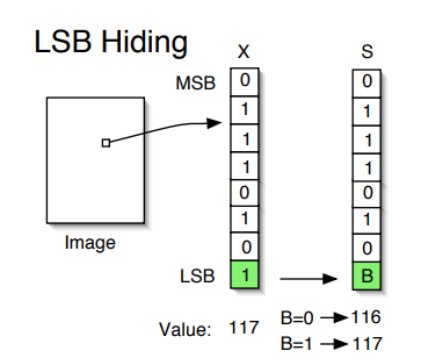
\includegraphics[width=0.6\textwidth]{graphics/chapter-3/lsb_hiding.PNG}
    \caption{Hình minh họa cho LSB}
    \label{fig:LSB}
\end{figure*}

\section{Video steganography trong thủy vân (watermarking)}

Trong phần này, chúng tôi trình bày 1 công cụ ẩn thông tin bao gồm 4 phương pháp để ẩn thông tin được biểu diễn chi tiết ở Hình \ref{tab:demo2_algo} trong miền biến đổi. 

\begin{figure}
    \centering
    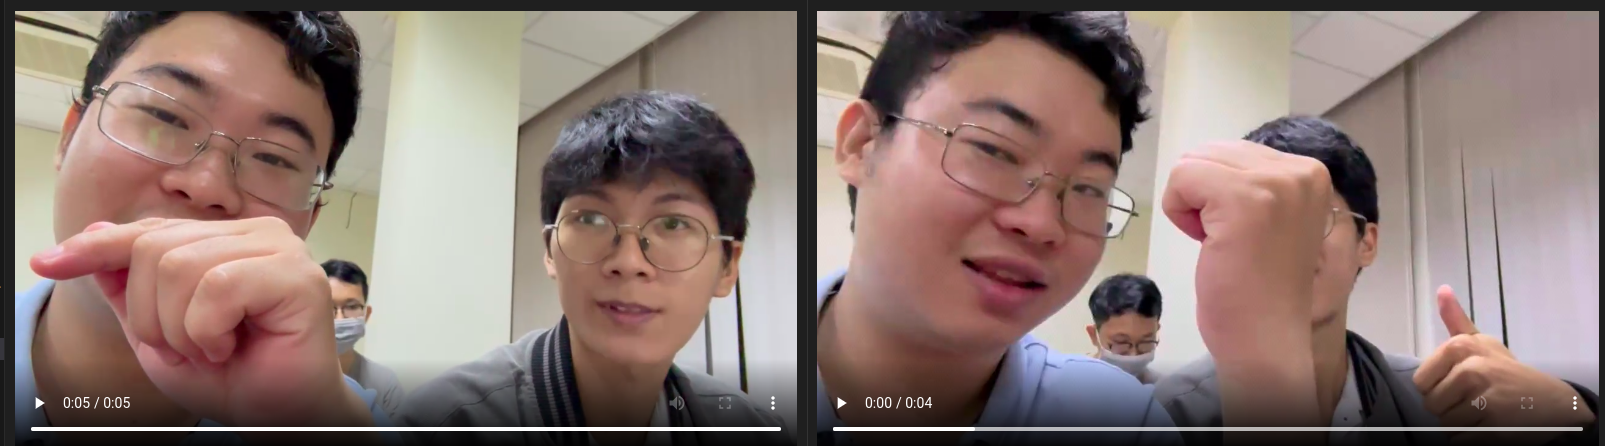
\includegraphics[scale=0.4]{graphics/chapter-3/chap3-video-hiding-video.png}
    \caption{Video trước (trái) và sau khi đã nhúng watermark}
    \label{fig:chap3-video-hiding-video}
\end{figure}


\begin{figure}
    \centering
    
\includegraphics[scale=0.4]{graphics/chapter-3/chap3-result-water-mark.png}
    \caption{Hình ảnh watermark sau khi trích xuất từ video (phải) và trước khi nhúng}
    \label{fig:chap3-result-water-mark}
\end{figure}

Công cụ này dựa trên thư viện Xuggler và được viết bằng Java để hỗ trợ đa nền tảng. Các thử nghiệm đã được thực hiện bằng cách nhúng vào các tệp định dạng .mp4 với codec H.264 và MPEG4 (phần mềm hỗ trợ tất cả các định dạng và codec được Xuggler hỗ trợ, tuy nhiên một số không phù hợp để nhúng).

\begin{table}[ht]
    \centering
    \caption{Bốn thuật toán sử dụng trong demo}
    \label{tab:demo2_algo}
    \begin{tabular}{| p{.25\textwidth} | p{.70\textwidth} |}
        \hline
        \textbf{Phương pháp} & \textbf{Mô tả}  \\
        \hline
        DCT \cite{algo1_kaur2011steganographic} & Phương pháp dựa trên việc nhúng dữ liệu vào các hệ số DCT 8 x 8 của một khung trong kênh Y của không gian màu YCbCr. Hai hệ số đã được chọn và so sánh – tùy thuộc vào hệ số nào có giá trị lớn hơn, giá trị 1 hoặc 0 được giải   mã. \\
        \hline
        DCT \cite{algo2_kothari2011performance} & Phương pháp tương tự như phương pháp DCT ở trên, nhưng sử dụng các hệ số khác nhau và hoạt động trên kênh G của không gian màu RGB. \\
        \hline
        DCT \cite{algo3_al2012robust} & Phương pháp dựa trên việc nhúng dữ liệu vào các hệ số khối 8 x 8 DCT bằng  cách sử dụng lượng tử hóa ghép nối và không ghép nối. Kênh G của không gian  màu RGB đã được sử dụng cho các thử nghiệm. $\delta$ cho thấy độ chính xác của lượng tử hóa. \\ 
        \hline
        DWT \cite{algo4_chetan2010dwt} & Phương pháp nhúng vào các vùng LL, HH và HL của phép biến đổi DWT. Kênh Y của không gian màu YCbCr được sử dụng trong phương pháp. \\
        \hline
    \end{tabular}
\end{table}

% \begin{table}[!h]
% \centering
% \caption{4 thuật toán sử dụng trong demo} 
% \label{tab:demo2_algo}
% \resizebox{\textwidth}{!}{
% \begin{tabular}{|c|c|}
% \hline
% \textbf{Phương pháp} &
%   \textbf{Mô tả} \\ \hline
% DCT \cite{algo1_kaur2011steganographic} &
%   \begin{tabular}[c]{@{}c@{}}Phương pháp dựa trên việc nhúng dữ liệu vào các hệ số DCT 8 x 8 của một \\ khung trong kênh Y của không gian màu YCbCr. Hai hệ số đã được chọn và so \\ sánh – tùy thuộc vào hệ số nào có giá trị lớn hơn, giá trị 1 hoặc 0 được giải   mã.\end{tabular} \\ \hline
% DCT \cite{algo2_kothari2011performance} &
%   \begin{tabular}[c]{@{}c@{}}Phương pháp tương tự như phương pháp DCT ở trên, nhưng sử dụng các hệ số\\  khác nhau và hoạt động trên kênh G của không gian màu RGB.\end{tabular} \\ \hline
% DCT \cite{algo3_al2012robust} &
%   \begin{tabular}[c]{@{}c@{}}Phương pháp dựa trên việc nhúng dữ liệu vào các hệ số khối 8 x 8 DCT bằng \\ cách sử dụng lượng tử hóa ghép nối và không ghép nối. Kênh G của không gian\\  màu RGB đã được sử dụng cho các thử nghiệm. Δ cho thấy độ chính xác của lượng   tử hóa.\end{tabular} \\ \hline
% DWT \cite{algo4_chetan2010dwt} &
%   \begin{tabular}[c]{@{}c@{}}Phương pháp nhúng vào các vùng LL, HH và HL của phép biến đổi DWT. Kênh Y \\ của không gian màu YCbCr được sử dụng trong phương pháp.\end{tabular} \\ \hline
% \end{tabular}
% }
% \end{table}

Trong nỗ lực không ngừng để tối ưu hóa việc ẩn giấu thông tin trong hình ảnh và video, chúng tôi đã sử dụng các thuật toán tiên tiến, chủ yếu dựa trên phương pháp biến tướng của Discrete Cosine Transforms (DCT) và Discrete Wavelet Transforms (DWT). Nhờ sự điều chỉnh tinh vi các hệ số và kênh màu (RGB hoặc YCbCr), chúng tôi đã xây dựng được một cơ chế mạnh mẽ để thực hiện việc ẩn các video vào các video khác.

Các hệ thống mã hóa thông tin đang dần trở nên thông minh hơn, và một phần quan trọng của điều này là việc thay đổi cách thông tin được biểu diễn trên hình ảnh. Hai loại kênh màu chính - RGB và YCbCr - đã chứng tỏ khả năng linh hoạt trong việc chuyển đổi giữa chúng thông qua những dòng mã lệnh được thiết kế cẩn thận. Điều này làm cho việc tạo ra hình ảnh và video mới kết hợp thông tin bí mật trở nên dễ dàng và hiệu quả hơn.

Mô hình màu RGB (Red Green Blue) là mô hình cơ bản dựa trên việc kết hợp ba màu cơ bản: đỏ, xanh lá cây và xanh dương. Mỗi pixel trong hình ảnh được biểu diễn bằng cách chỉ định giá trị của ba kênh màu này. Mô hình RGB phản ánh cách con người cảm nhận màu sắc thông qua ba màu cơ bản này. Mặc dù dễ dàng hiểu và có thể biểu diễn trực tiếp các màu sắc cơ bản, tuy nhiên, mô hình này không phản ánh một cách chính xác khả năng nhận biết màu sắc của mắt người. Thường không thích hợp cho việc xử lý và nén hình ảnh.

Trái với đó, mô hình màu YCbCr (Luminance Chrominance) chia thành ba kênh: Y biểu diễn thông tin về độ sáng của điểm ảnh, trong khi Cb và Cr biểu diễn thông tin về màu sắc. Mô hình YCbCr thể hiện tốt hơn khả năng nhận biết màu sắc của mắt người, điều này khiến nó phù hợp cho việc xử lý hình ảnh, nén và truyền tải qua các kênh có băng thông hạn chế. Tính chất này đặc biệt hữu ích khi cần tách biệt thông tin độ sáng và thông tin màu sắc để thực hiện các phép biến đổi hoặc giảm dung lượng dữ liệu.

Mặc dù YCbCr có nhiều ưu điểm trong việc xử lý hình ảnh, việc chuyển đổi giữa RGB và YCbCr vẫn cần thiết khi cần hiển thị trực tiếp trên các thiết bị RGB. Nhưng với khả năng tách biệt thông tin màu sắc và độ sáng, YCbCr vẫn là một lựa chọn phổ biến trong việc xử lý hình ảnh và video để đảm bảo chất lượng và khả năng nhận biết màu sắc tốt hơn.

Discrete Cosine Transforms (DCT) là một phương pháp biến đổi tín hiệu từ miền thời gian sang miền tần số. Đặc biệt, DCT chia tín hiệu thành các khung nhỏ, sau đó biến đổi mỗi khung bằng cách tính tổ hợp tuyến tính của các hàm cosin với các tần số khác nhau. Kết quả là một tập hệ số DCT thể hiện mức độ xuất hiện của các tần số trong từng khung. DCT thường được áp dụng rộng rãi trong nhiều lĩnh vực như nén hình ảnh (ví dụ: định dạng JPEG) và nén âm thanh (ví dụ: định dạng MP3). Hơn nữa, DCT còn được áp dụng trong việc ẩn thông tin, khi thông tin bí mật được nhúng vào các hệ số tần số thấp, mà mắt người ít nhạy cảm.

Tổng cộng, việc sử dụng các phương pháp biến đổi như DCT và tận dụng các mô hình biểu diễn màu sắc như RGB và YCbCr đã đóng một vai trò quan trọng trong việc tối ưu hóa quá trình ẩn thông tin và xử lý hình ảnh. Việc lựa chọn kỹ thuật phù hợp sẽ phụ thuộc vào mục tiêu cụ thể của ứng dụng và yêu cầu về chất lượng.


\begin{figure*}[!h]
    \centering
    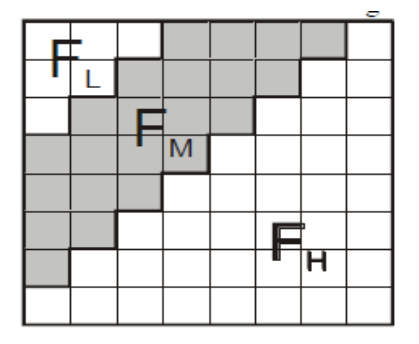
\includegraphics[width=0.6\textwidth]{graphics/chapter-3/DCT_algo1.PNG}
    \caption{Hình minh họa cho DCT}
    \label{fig:PNG}
\end{figure*}

DWT là một phương pháp biến đổi tín hiệu thành các thành phần sóng con ở các tần số và độ phân giải khác nhau. Thay vì sử dụng các hàm cosin như DCT, DWT thực hiện biến đổi bằng cách sử dụng các bộ lọc sóng con. Tín hiệu được phân tách thành các thành phần sóng con ở các tần số thấp và cao, cùng với các mức độ phân giải khác nhau. DWT thường được sử dụng trong nhiều ứng dụng như nén hình ảnh (Wavelet-based image compression) và phân tích tín hiệu y tế. Cũng như DCT, DWT có khả năng ẩn thông tin bằng cách chèn dữ liệu vào các thành phần sóng con thấp tần số hoặc thấp độ phân giải.

\begin{figure*}[!h]
    \centering
    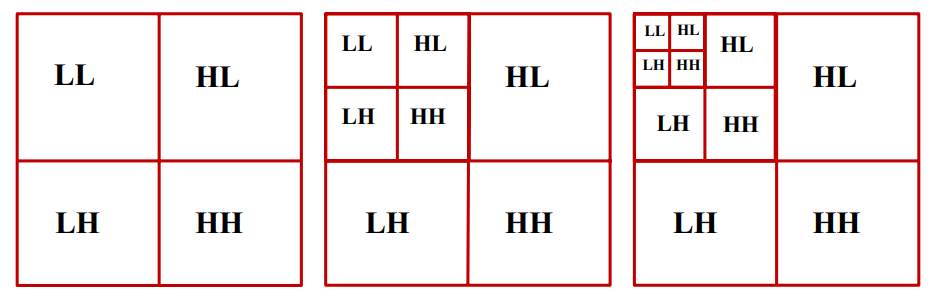
\includegraphics[width=0.6\textwidth]{graphics/chapter-3/DWT.PNG}
    \caption{Hình minh họa cho DWT}
    \label{fig:PNG}
\end{figure*}


\section{Video steganography sử dụng học máy}
Trong phần này, chúng tôi chứng tỏ sự tinh vi và đột phá của một mạng thần kinh tích chập tiên tiến, thường được gọi là convolutional neural network, nhằm mục đích tối ưu hóa việc ẩn những video trong video. Nhiệm vụ đặc biệt quan trọng mà chúng tôi đã đặt ra là ẩn đi một hình ảnh màu có kích thước to lớn (N*N RGB) vào trong một bức tranh khác cùng kích thước. Qua quá trình đào tạo mạng lưới neural sâu song song, chúng tôi đã xây dựng một cặp quy trình quan trọng: quá trình mã hóa và quá trình giải mã, hai khía cạnh này hoạt động như một đôi hoàn thiện nhau. Tại cốt lõi của kỹ thuật này là khả năng nén hình ảnh thông qua việc sử dụng các mạng mã hóa tự động (auto-encoding networks). Toàn bộ hệ thống đã được đào tạo để "học" cách chuyển đổi thông tin từ hình ảnh bí mật vào những phần ít được chú ý nhất trong hình ảnh chứa, và sau đó "học" cách khôi phục và tái tạo thông tin tương tự từ hình ảnh chứa này. Mục tiêu là thực hiện việc mã hóa thông tin một cách hiệu quả, đồng thời giảm thiểu tổn thất dữ liệu.

Chúng tôi đã thực hiện quá trình đào tạo một bộ cặp mạng ẩn và hiển thị đồng thời, sử dụng mô hình bộ mã hóa tự động và sử dụng thư viện Keras để hỗ trợ cho quá trình này. Mô hình này bao gồm hai lớp đầu vào, mỗi lớp tương ứng với một cặp hình ảnh gồm hình ảnh bí mật và hình ảnh bao quanh, và có hai lớp đầu ra tương ứng với đầu vào của chúng. Do mô hình dựa trên kiến trúc mã hóa tự động, việc gán nhãn trong quá trình đào tạo phải tương ứng với đầu vào của nó.

Kiến trúc mạng neural của chúng tôi bao gồm ba phần cốt lõi: Phần Chuẩn bị (Prepare block), Phần Ẩn (Hide block) và Phần Tiết lộ (Reveal block). Trong phần Chuẩn bị, chúng tôi đã thực hiện việc biến đổi các điểm ảnh màu ban đầu thành những đặc trưng có ý nghĩa cao hơn, giúp việc mã hóa hình ảnh trở nên dễ dàng và hiệu quả hơn. Tiếp theo, chúng tôi đã tiến hành việc ẩn hình ảnh đã được biến đổi vào trong hình ảnh bao quanh thông qua sự áp dụng của Phần Ẩn, tạo ra một hình ảnh vùng chứa (container image) đặc biệt. Cuối cùng, trong Phần Tiết lộ, chúng tôi đã thực hiện việc giải mã hình ảnh vùng chứa để tạo ra đầu ra bí mật ban đầu, đảm bảo rằng thông tin quý báu được khôi phục một cách chính xác. Do đó, biểu đồ huấn luyện ở hình \ref{fig:train_graph} có hai đầu vào và hai đầu ra.

\begin{figure*}[!h]
    \centering
    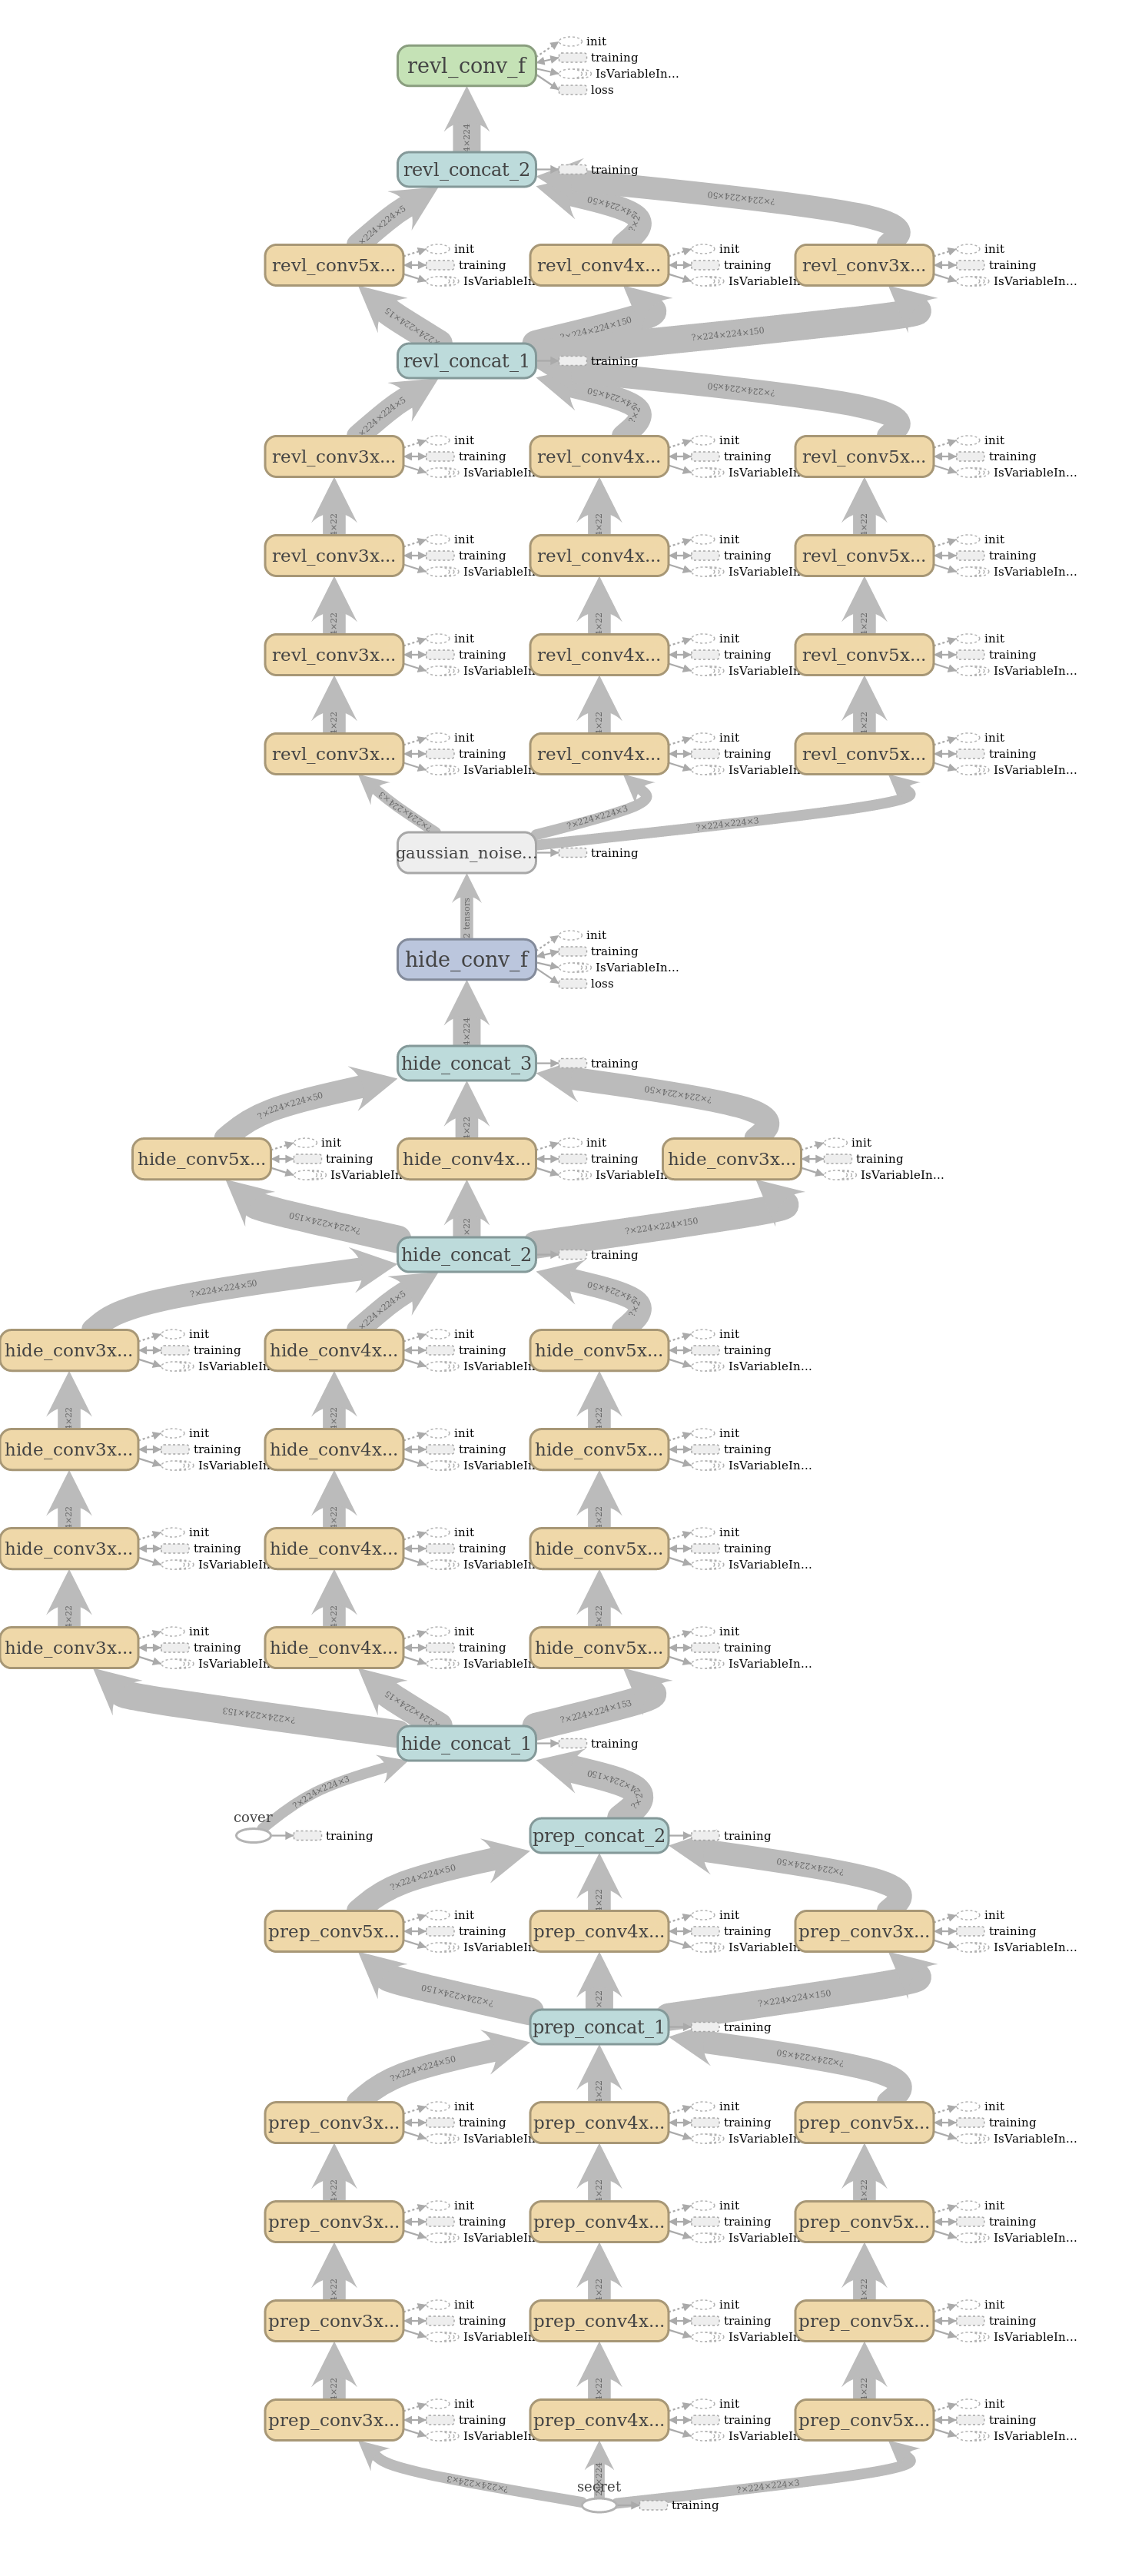
\includegraphics[width=0.6\textwidth]{graphics/chapter-3/train_graph.png}
    \caption{Biểu đồ huấn luyện của mô hình mạng tích chập}
    \label{fig:train_graph}
\end{figure*}


Chúng tôi sử dụng hàm \textbf{weighted L2 loss} và \textbf{Adam optimizer} để huấn luyện mô hình.

Để đảm bảo rằng các mạng không chỉ mã hóa hình ảnh bí mật trong LSB, một lượng nhiễu nhỏ được thêm vào đầu ra của mạng thứ hai (ví dụ: vào hình ảnh vùng chứa được tạo) trong quá trình đào tạo.

Sau khi đào tạo, chúng tôi chia mô hình được đào tạo thành hai: mạng mã hóa và mạng giải mã (chúng tôi loại bỏ lớp nhiễu). Mạng ẩn có hai đầu vào tương ứng với ảnh bí mật và ảnh bìa và một đầu ra tương ứng với ảnh vùng chứa (container image). Mạng giải mã lấy hình ảnh vùng chứa làm đầu vào và tiết lộ (giải mã) hình ảnh bí mật làm đầu ra.

Mạng giải mã được sử dụng bởi người gửi; trong khi mạng mã hóa được dùng bởi người nhận. Người nhận chỉ có quyền truy cập vào hình ảnh vùng chứa. 

Trong video, video sẽ được tách thành các frame nhỏ và mô hình sẽ xử lý 4 frame 1 lần.


\begin{figure}
    \centering
    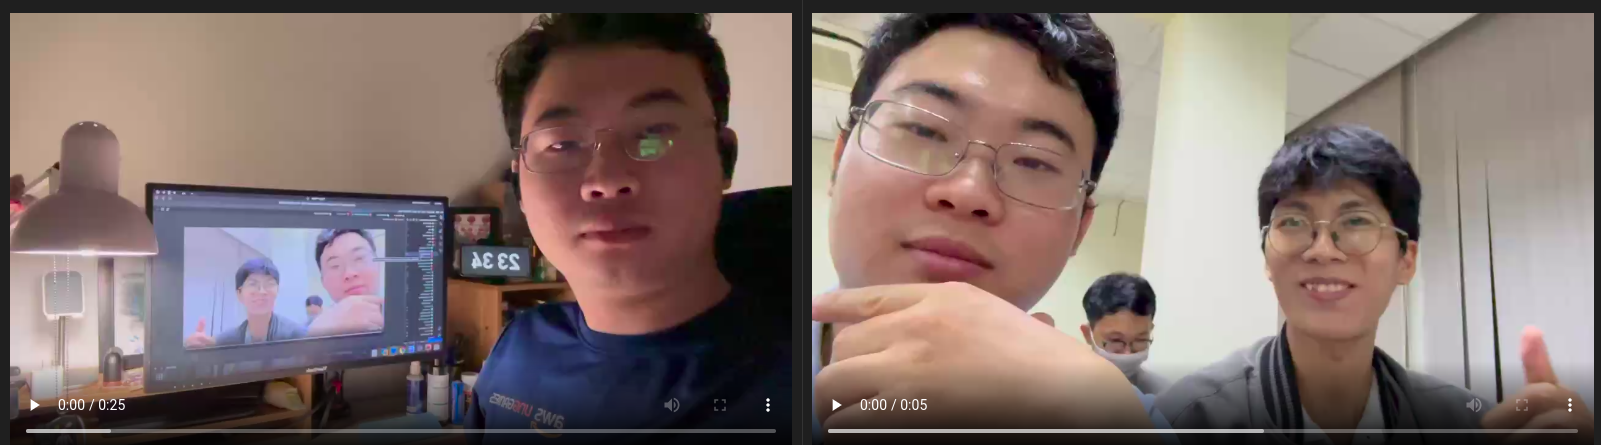
\includegraphics[scale=0.4]{graphics/chapter-3/chap3-video-hiding-to-video.png}
    \caption{Cover video (trái) và video secret muốn ẩn vào trong cover}
    \label{fig:chap3-video-hiding-to-video}
\end{figure}

\begin{figure}
    \centering
    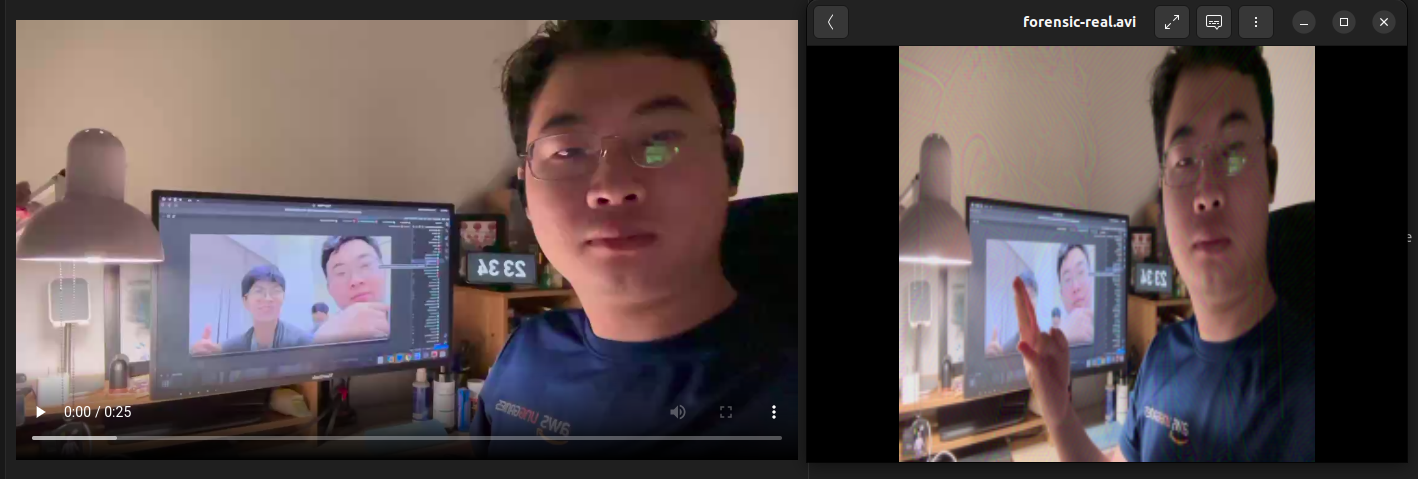
\includegraphics[scale=0.4]{graphics/chapter-3/chap3-video-after-hiding.png}
    \caption{Video trước (trái) và sau khi đã nhúng một video khác vào}
    \label{fig:enter-label}
\end{figure}
% \include{chapters/main/chapter-4.tex}
% \include{chapters/main/chapter-5.tex}
% % Print references
\fancyhf{}
\printbibliography[heading=bibintoc, title = {Tài liệu tham khảo}]
\end{document}
